%!TEX root = ./aistats_2019_sketchmcmc_supp.tex


% \section{Visual Comparison with Existing Approaches}

% In this section, we provide the results presented in \cite{deshpande2018generative} for visual comparison. These results are obtained by running different IGM approaches on the MNIST dataset, namely GAN \cite{goodfellow2014generative}, Wasserstein GAN (W-GAN) \cite{arjovsky2017wasserstein} and the Sliced-Wasserstein Generator (SWG) \cite{deshpande2018generative}.

% \begin{figure}[h!]
% \centering
% 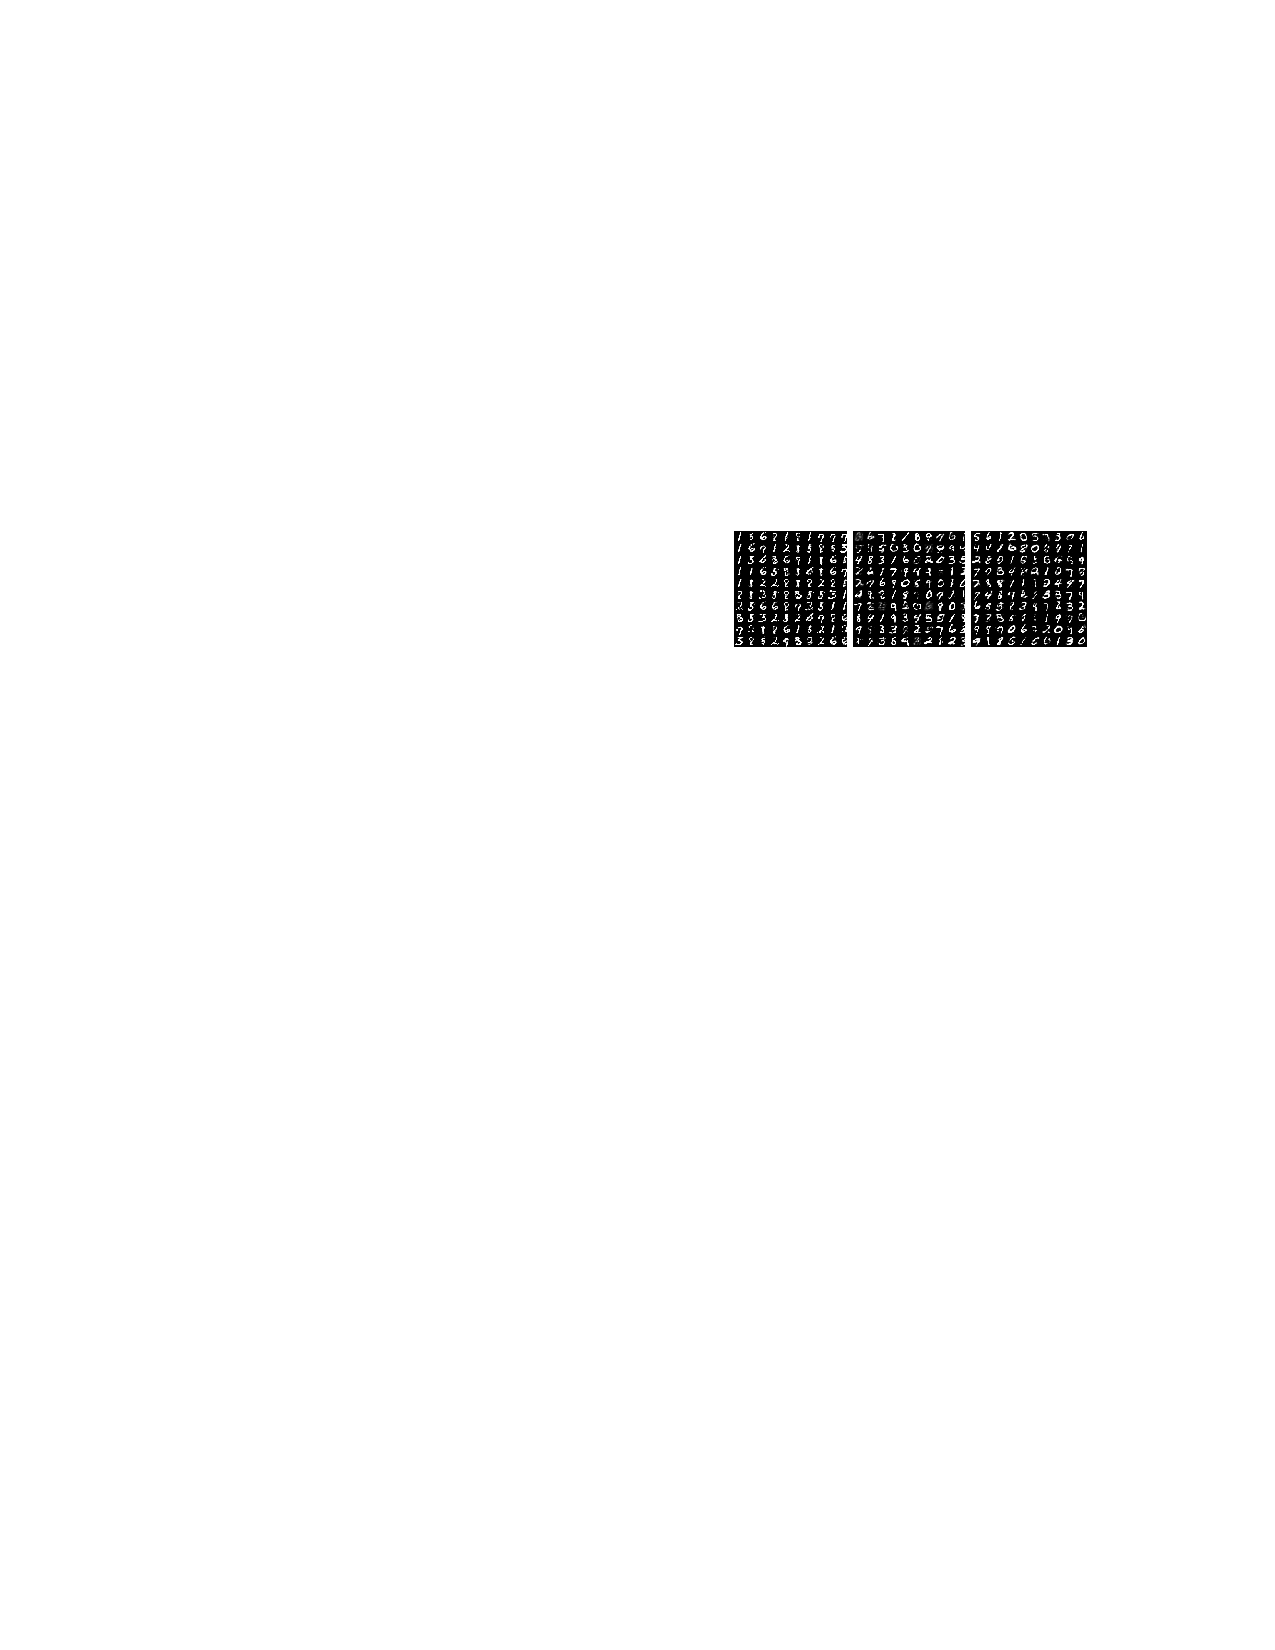
\includegraphics[width=0.5\columnwidth]{mnist_all.pdf}
% \caption{Performance of GAN (left), W-GAN (middle), SWG (right) on MNIST. (The figure is directly taken from \cite{deshpande2018generative}.) }
% \label{fig:mnistall}
% \end{figure}


\section{Additional Experimental Results}

\subsection{The Sliced Wasserstein Flow}
The whole code for the Sliced Wasserstein Flow was implemented in Python, for use with Pytorch\footnote{\url{http://www.pytorch.org}.}. The code was written so as to run efficiently on GPU, and is available on the publicly available repository related to this paper\footnote{\url{https://github.com/aliutkus/swf}.}.

In practice, the SWF involves relatively simple operations, the most important being:
\begin{itemize}
  \item For each random $\theta\in\{\theta_n\}_{n=1\dots N_\theta}$,  compute its inner product with all items from a dataset and obtain the empirical quantiles for these \emph{projections}.
  \item At each step $k$ of the SWF, for each projection $z=\left<\theta, \bar{X}^i_k\right>$, apply two piece-wise linear functions, corresponding to the scalar optimal transport $\psi_{k, \theta}'(z)$.
\end{itemize}
Even if such steps are conceptually simple, the quantile and required linear interpolation functions were not available on GPU for any framework we could figure out at the time of writing this paper. Hence, we implemented them ourselves for use with Pytorch, and the interested reader will find the details in the Github repository dedicated to this paper.

Given these operations, putting a SWF implementation together is straightforward.
The code provided allows not only to apply it on any dataset, but also provides routines to have the computation of these sketches running in the background in a parallel manner.

\subsection{The need for dimension reduction through autoencoders}

In this study, we used an autoencoder trained on the dataset as a dimension reduction technique, so that the SWF is applied to transport particles in a latent space of dimension $d\approx 50$, instead of the original $d>1000$ of image data.

The curious reader may wonder why SWF is not applied directly to this original space, and what performances should be expected there. We have done this experiment, and we found out that SWF has much trouble rapidly converging to satisfying samples. In figure~\ref{fig:suppnoae}, we show the progressive evolution of particles undergoing SWF when the target is directly taken as the uncompressed dataset.

\begin{figure}
\centering
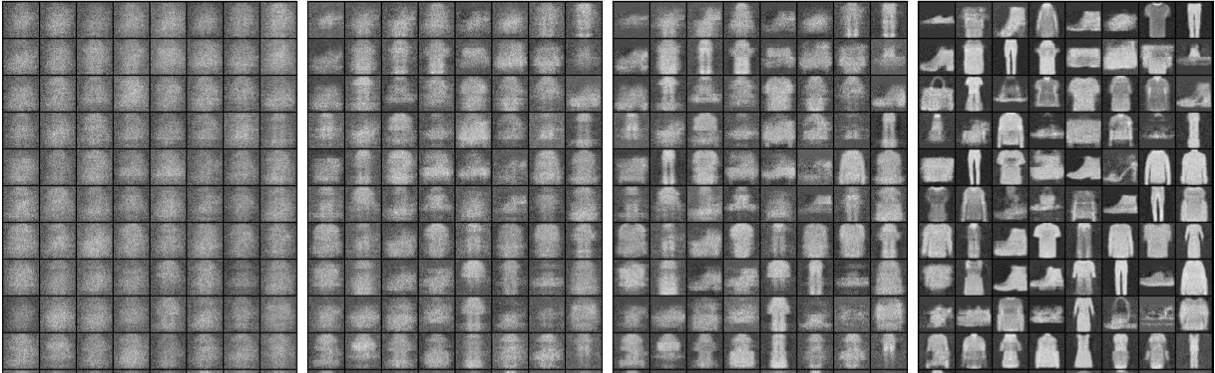
\includegraphics[width=\columnwidth]{figures/supplementary/fmnist.png}
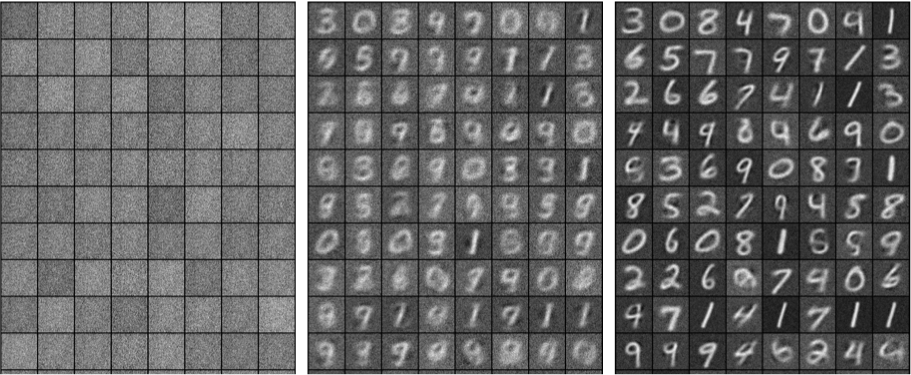
\includegraphics[width=\columnwidth]{figures/supplementary/mnist.png}
\caption{The evolution of SWF through 15000 iterations, when the original high-dimensional data is kept instead of working on reduced bottleneck features as done in the main document. Showing results on the MNIST and FashionMNIST datasets. For a visual comparison for FashionMNIST, we refer the reader to \cite{samangouei2018defensegan}.}
\label{fig:suppnoae}
\end{figure}

In this experiment, the strategy was to change the projections $\theta$ at each iteration, so that we ended up with a set of projections being $\{\theta_{n,k}\}_{n=1\dots N_\theta}^{k=1\dots K}$ instead of the fixed set of $N_\theta$ we now consider in the main document (for this, we picked $N_\theta=200$). This strategy is motivated by the complete failure we observed whenever we picked such fixed projections throughout iterations, even for a relatively large number as $N_\theta=16000$.

As may be seen on Figure~\ref{fig:suppnoae}, the particles definitely converge to samples from the desired datasets, and this is encouraging. However, we feel that the extreme number of iterations required to achieve such convergence comes from the fact that theory needs an integral over the $d-$dimensional sphere at each step of the SWF, which is clearly an issue whenever $d$ gets too large.
Although our solution of picking new samples from the sphere at each iteration alleviated this issue to some extent, the curse of dimensionality prevents us from doing much better with just thousands of \emph{random} projections at a time.

This being said, we are confident that good performance would be obtained if millions of random projections could be considered for transporting such high dimensional data because i/ theory suggests it and ii/ we observed excellent performance on reduced dimensions.

However, we, unfortunately, did not have the computing power it takes for such large scale experiments and this is what motivated us in the first place to introduce some dimension-reduction technique through AE.

\subsection{Structure of our autoencoders for reducing data dimension}

As mentioned in the text, we used autoencoders to reduce the dimensionality of the transport problem. The structure of these networks is the following:

\begin{itemize}
  \item $\textbf{Encoder}$ Four 2d convolution layers with (num\_chan\_out, kernel\_size, stride, padding) being $(3,3,1,1)$, $(32,2,2,0)$, $(32,3,1,1)$, $(32, 3,1,1)$, each one followed by a ReLU activation. At the output, a linear layer gets the desired bottleneck size.

  \item $\textbf{Decoder}$ A linear layer gets from the bottleneck features to a vector of dimension $8192$, which is reshaped as $(32, 16,16)$. Then, three convolution layers are applied, all with $32$ output channels and (kernel\_size, stride, panning) being respectively $(3,1,1)$, $(3,1,1)$, $(2,2,0)$. A 2d convolution layer is then applied with an output number of channels being that of the data ($1$ for black and white, $3$ for color), and a (kernel\_size, stride, panning) as $(3,1,1)$. In any case, all layers are followed by a ReLU activation, and a sigmoid activation is applied a the very output.
\end{itemize}

Once these networks defined, these autoencoders are trained in a very simple manner by minimizing the binary cross entropy between input and output over the training set of the considered dataset (here MNIST, CelebA or FashionMNIST). This training was achieved with the Adam algorithm \cite{kingma2014adam} with learning rate $1e-3$.

No additional training trick was involved as in Variational Autoencoder \cite{kingma2013VAE} to make sure the distribution of the bottleneck features matches some prior. The core advantage of the proposed method in this respect is indeed to turn any previously learned AE as a generative model, by automatically and non-parametrically transporting particles drawn from an arbitrary prior distribution $\mu$ to the observed empirical distribution $\nu$ of the bottleneck features over the training set.

\subsection{Convergence plots of SWF}

\begin{figure}
\begin{centering}
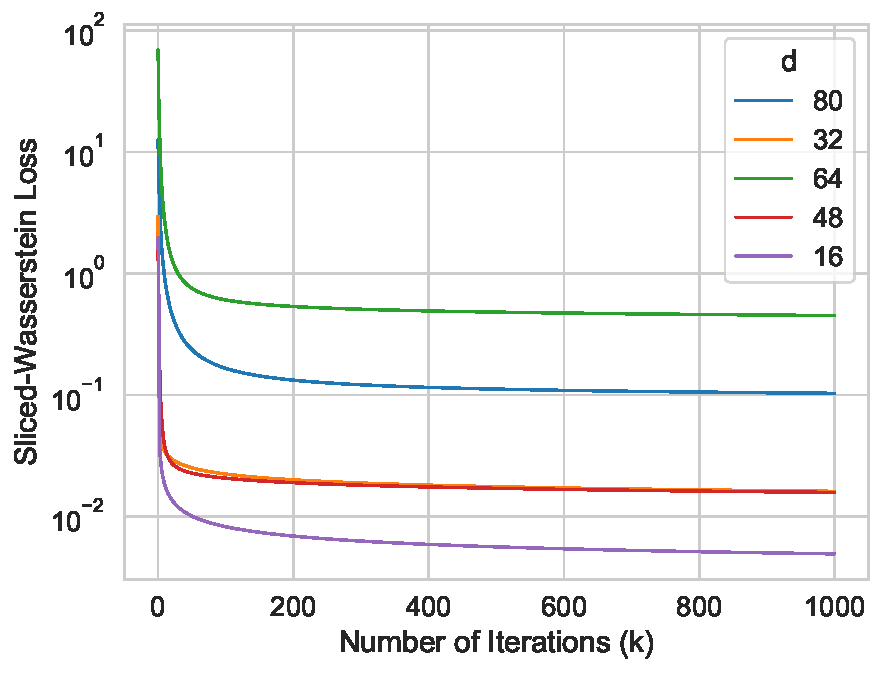
\includegraphics[width=0.5\columnwidth]{figures/iterations.pdf}
\par\end{centering}
\caption{Approximately computed $\SW$ between the output $\bar{\mu}_{k}^{N}$ and data distribution $\nu$ in the MNIST experiment for different dimensions $d$ for the bottleneck features (and the corresponding pre-trained AE).
\label{fig:supptoy_sw}}
\end{figure}

In the same experimental setting as in the main document, we also illustrate the behavior of the algorithm for varying dimensionality $d$ for the bottleneck-features. To monitor the convergence of SWF as predicted by theory, we display the approximately computed $\SW$ distance between the distribution of the particles and the data distribution. Even though minimizing this distance is not the real objective of our method, arguably, it is still a good proxy for understanding the convergence behavior.

Figure~\ref{fig:supptoy_sw} illustrates the results. We observe that, for all choices of $d$, we see a steady and smooth decrease in the cost for all runs, which is in line with our theory. The absolute value of the cost for varying dimensions remains hard to interpret at this stage of our investigations.

\section{Additional samples}

\subsection{Evolution throughout iterations}

In Figures~\ref{fig:suppmnist} and \ref{fig:suppfmnist} below, we provide the evolution of the SWF algorithm on the Fashion MNIST and the MNIST datasets in higher resolution, for an AE with $d=48$ bottleneck features.

\newcommand{\picwidth}{0.2}%originally 0.24
\begin{figure}
\centering
\includegraphics[width=\picwidth\columnwidth]{supplementary/mnist/train_image_0.png}
\includegraphics[width=\picwidth\columnwidth]{supplementary/mnist/train_image_10.png}
\includegraphics[width=\picwidth\columnwidth]{supplementary/mnist/train_image_20.png}
\includegraphics[width=\picwidth\columnwidth]{supplementary/mnist/train_image_30.png}\\
\includegraphics[width=\picwidth\columnwidth]{supplementary/mnist/train_image_40.png}
\includegraphics[width=\picwidth\columnwidth]{supplementary/mnist/train_image_50.png}
\includegraphics[width=\picwidth\columnwidth]{supplementary/mnist/train_image_100.png}
\includegraphics[width=\picwidth\columnwidth]{supplementary/mnist/train_image_200.png}
\caption{The evolution of SWF through 200 iterations on the MNIST dataset. Plots are for $1$, $11$, $21$, $31$, $41$, $51$, $101$ and $201$ iterations}
\label{fig:suppmnist}
\end{figure}

\begin{figure}
\centering
\includegraphics[width=\picwidth\columnwidth, frame]{supplementary/alternative_fmnist/train_image_0.png}%
\includegraphics[width=\picwidth\columnwidth, frame]{supplementary/alternative_fmnist/train_image_10.png}%
\includegraphics[width=\picwidth\columnwidth, frame]{supplementary/alternative_fmnist/train_image_20.png}%
\includegraphics[width=\picwidth\columnwidth, frame]{supplementary/alternative_fmnist/train_image_30.png}\\%
\includegraphics[width=\picwidth\columnwidth, frame]{supplementary/alternative_fmnist/train_image_40.png}%
\includegraphics[width=\picwidth\columnwidth, frame]{supplementary/alternative_fmnist/train_image_50.png}%
\includegraphics[width=\picwidth\columnwidth, frame]{supplementary/alternative_fmnist/train_image_100.png}%
\includegraphics[width=\picwidth\columnwidth, frame]{supplementary/alternative_fmnist/train_image_200.png}%
\caption{The evolution of SWF through 200 iterations on the FashionMNIST dataset. Plots are for $1$, $11$, $21$, $31$ (upper row) and $41$, $51$, $101$, $201$ (lower row) iterations}
\label{fig:suppfmnist}
\end{figure}

\subsection{Training samples, interpolation and extrapolation}

In Figures~\ref{fig:suppmnistsamples} and \ref{fig:suppfmnistsamples} below, we provide other examples of outcome from SWF, both for the MNIST and the FashionMNIST datasets, still with $d=48$ bottleneck features.

The most noticeable fact we may see on these figures is that while the actual particles which went through SWF, as well as linear combinations of them, all yield very satisfying results, this is however not the case for particles that are drawn randomly and then brought through a pre-learned SWF.

Once again, we interpret this fact through the curse of dimensionality: while we saw in our toy GMM example that using a pre-trained SWF was totally working for small dimensions, it is already not so for $d=48$ and only $3000$ training samples.

This noticed, we highlight that this generalization weakness of SWF for high dimensions is not really an issue, since it is always possible to i/ run SWF with more training samples if generalization is required ii/ re-run the algorithm for a set of new particles. Remember indeed that this does not require passing through the data again, since the distribution of the data projections needs to be done only once.
\renewcommand{\picwidth}{0.3}%originally 0.24


\begin{figure}
\centering
\subfigure[particles undergoing SWF]{
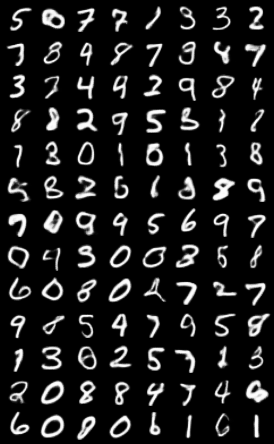
\includegraphics[width=\picwidth\columnwidth]{supplementary/MNIST_train_image_1000.png}}
\subfigure[After SWF is done: applying learned map on linear combinations of train particles]{
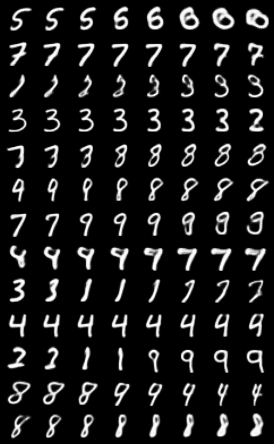
\includegraphics[width=\picwidth\columnwidth]{supplementary/MNIST_interp_image_1000.png}}
\subfigure[After SWF is done: applying learned map on random inputs.]{
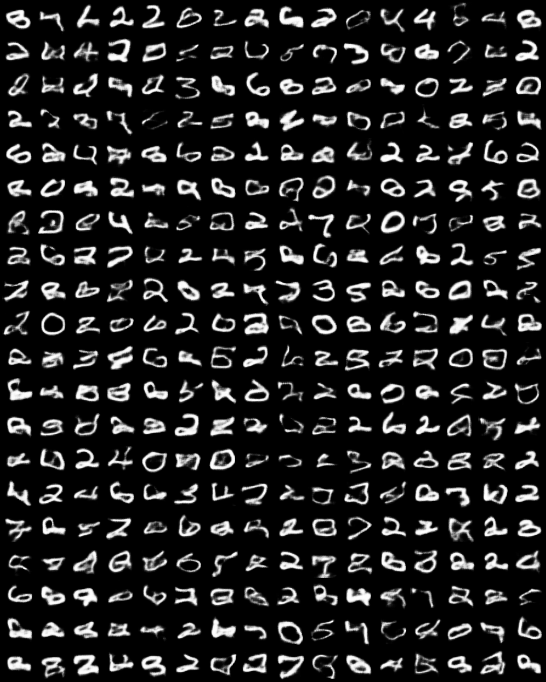
\includegraphics[width=\picwidth\columnwidth]{supplementary/MNIST_randomtest_image_1000.png}}
\caption{SWF on MNIST: training samples, interpolation in learned mapping, extrapolation.}
\label{fig:suppmnistsamples}
\end{figure}


\begin{figure}
\centering
\subfigure[particles undergoing SWF]{
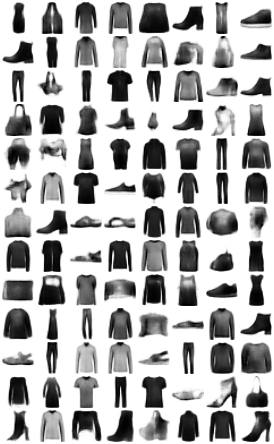
\includegraphics[width=\picwidth\columnwidth]{supplementary/FashionMNIST_train_image_1000.png}}
\subfigure[After SWF is done: applying learned map on linear combinations of train particles]{
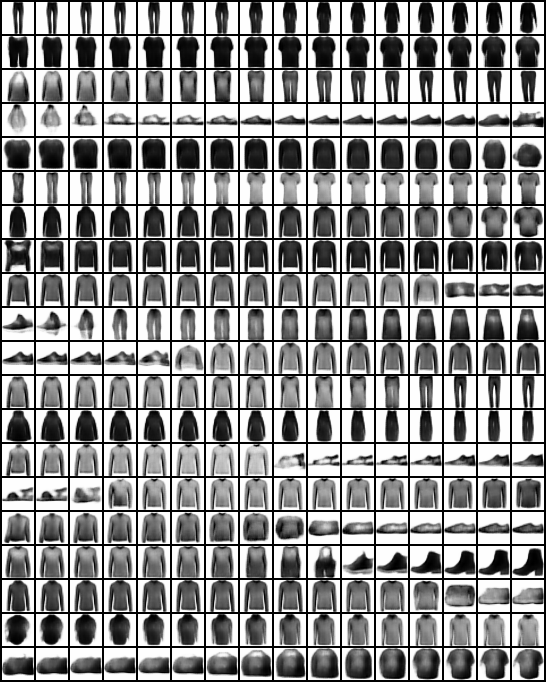
\includegraphics[width=\picwidth\columnwidth]{supplementary/FashionMNIST_interp_image_1000.png}}
\subfigure[After SWF is done: applying learned map on random inputs.]{
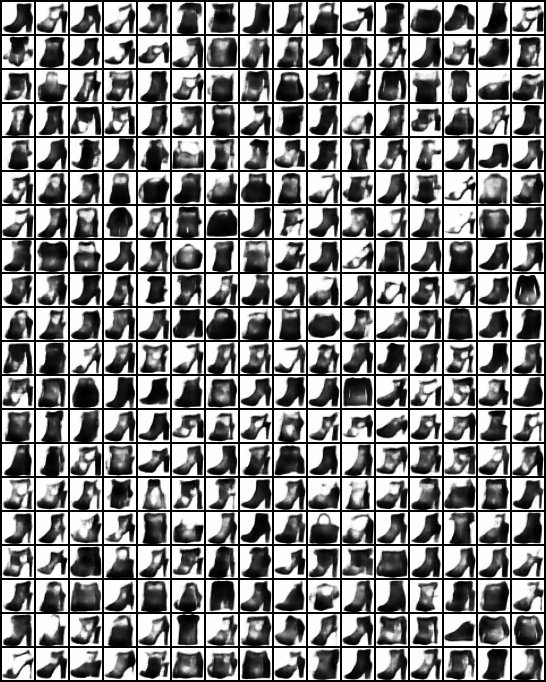
\includegraphics[width=\picwidth\columnwidth]{supplementary/FashionMNIST_randomtest_image_1000.png}}
\caption{SWF on FashionMNIST: training samples, interpolation in learned mapping, extrapolation.}
\label{fig:suppfmnistsamples}
\end{figure}







% \section{Details of Computing $(F_{\theta_{n}^*\#\hat{\mu}}^{-1} \circ F_{\theta^*_{n}\#\nu}) $}


% \umut{Antoine. -- sorting, interpolation etc}

% \begin{figure}
% \begin{centering}
% \setlength\tabcolsep{1pt}
% \begin{tabular}{cccccc}
% $\lambda=0$ & $\lambda=0.1$ & $\lambda=0.2$ & $\lambda=0.3$ & $\lambda=0.5$ & $\lambda=1$\tabularnewline
% 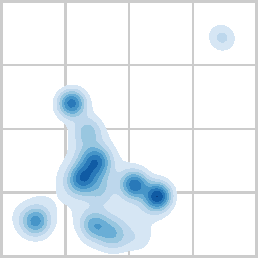
\includegraphics[width=2cm]{figures/supplementary/regularization/r0_output_dist_k=70-crop.pdf} & 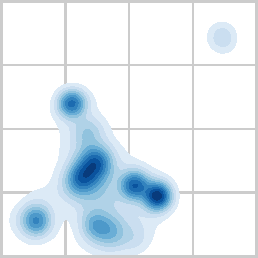
\includegraphics[width=2cm]{figures/supplementary/regularization/r01_output_dist_k=70-crop.pdf} & 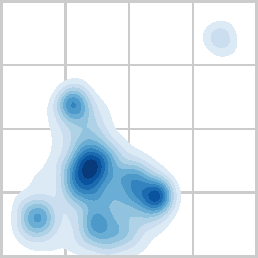
\includegraphics[width=2cm]{figures/supplementary/regularization/r02_output_dist_k=70-crop.pdf} &  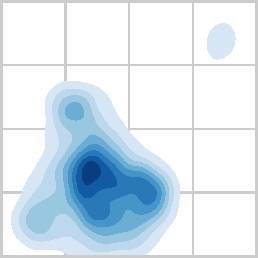
\includegraphics[width=2cm]{figures/supplementary/regularization/r03_output_dist_k=70-crop.pdf}&  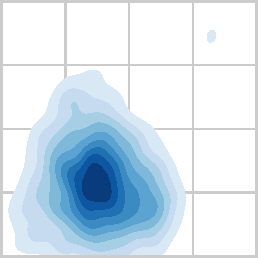
\includegraphics[width=2cm]{figures/supplementary/regularization/r05_output_dist_k=70-crop.pdf} &  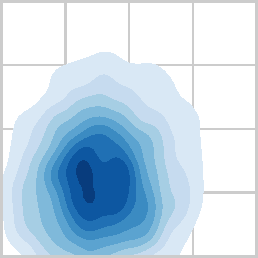
\includegraphics[width=2cm]{figures/supplementary/regularization/r1_output_dist_k=70-crop.pdf}
% \end{tabular}
% \par\end{centering}
% \caption{Influence of the regularization parameter $\lambda$. The higher $\lambda$, the more entropic the output distribution.\label{fig:lambda_supp}}
% \end{figure}
